\documentclass[11pt,letterpaper]{article}
\usepackage{fullpage}
\usepackage{datetime}
\usepackage[pdftex]{graphicx}
\usepackage{amsfonts,eucal,amsbsy,amsopn,amsmath}
\usepackage{url}
\usepackage[sort&compress]{natbib}
\usepackage{natbibspacing}
\usepackage{latexsym}
\usepackage{wasysym} 
\usepackage{rotating}
\usepackage{fancyhdr}
\DeclareMathOperator*{\argmax}{argmax}
\DeclareMathOperator*{\argmin}{argmin}
\usepackage{sectsty}
\usepackage[dvipsnames,usenames]{color}
\usepackage{multicol}
\definecolor{orange}{rgb}{1,0.5,0}
\usepackage{multirow}
\usepackage{sidecap}
\usepackage{caption}
\renewcommand{\captionfont}{\small}
\setlength{\oddsidemargin}{-0.04cm}
\setlength{\textwidth}{16.59cm}
\setlength{\topmargin}{-0.04cm}
\setlength{\headheight}{0in}
\setlength{\headsep}{0in}
\setlength{\textheight}{22.94cm}
\allsectionsfont{\normalsize}
\newcommand{\ignore}[1]{}
\newenvironment{enumeratesquish}{\begin{list}{\addtocounter{enumi}{1}\arabic{enumi}.}{\setlength{\itemsep}{-0.25em}\setlength{\leftmargin}{1em}\addtolength{\leftmargin}{\labelsep}}}{\end{list}}
\newenvironment{itemizesquish}{\begin{list}{\setcounter{enumi}{0}\labelitemi}{\setlength{\itemsep}{-0.25em}\setlength{\labelwidth}{0.5em}\setlength{\leftmargin}{\labelwidth}\addtolength{\leftmargin}{\labelsep}}}{\end{list}}

\bibpunct{(}{)}{;}{a}{,}{,}
\newcommand{\nascomment}[1]{\textcolor{blue}{\textbf{[#1 --NAS]}}}


\pagestyle{fancy}
\lhead{}
\chead{}
\rhead{}
\lfoot{}
\cfoot{\thepage~of \pageref{lastpage}}
\rfoot{}
\renewcommand{\headrulewidth}{0pt}
\renewcommand{\footrulewidth}{0pt}


\title{11-712:  NLP Lab Report}
\author{Rajarshi Das}
\date{\today}

\begin{document}
\maketitle
\begin{abstract}
%\nascomment{one paragraph here summarizing what the paper is about}
\noindent This is a report on the development of an open source dependency parser for the language, Bengali. Presently I have reported some basic information about the language.
\end{abstract}

\noindent The goal of this project is to design, implement and evaluate a dependency parser for the language, Bengali (also my native language). This language is characterized by a rich system of inflections, derivation and compound formation \citep{saha2004computer,chakroborty2003uchchotoro} which makes analysis and generation of Bengali, a challenging task \citep{ghosh2009dependency}.

\section{Basic Information about Bengali}
According to \citep{ethnologue}, Bengali is an eastern Indo-Aryan Language and is native to the region of eastern south Asia. It is the official language of Bangladesh and is also spoken in the Indian state of West Bengal and parts of Tripura and Assam.\\

\noindent Bengali follows the SOV order in terms of ordering of subject, object and verb \citep{Dasgupta-2003}. It makes use of postpositions instead of prepositions. Determiners follow the noun while numerals, adjectives and possessors precede the noun. It exhibits no case or number agreement and no grammatical gender phenomena \citep{Dasgupta-2003}. Nouns and pronouns are declined into four cases - nominative, objective, genitive and locative \citep{Bhattacharya}\\

\noindent Bengali is written using the Bengali script. It has 11 vowel graphemes and 39 graphemes representing consonants and other modifiers. The script is written and read horizontally from left to right. Figure~\ref{vowels} and ~\ref{cons} show the vowels (and its  various diacritics) and consonants in the Bengali script (Image source: Internet).
\graphicspath{ {images/} }
\begin{figure}[h]
  \caption{Vowels and vowel diacritics in Bengali script.}
  \centering
  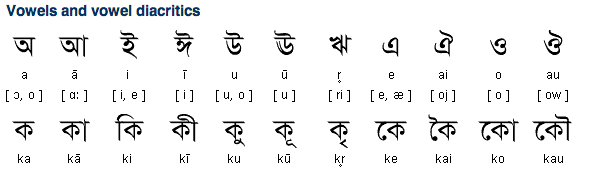
\includegraphics[scale=0.35]{vowels}
  \label{vowels}
\end{figure}
\begin{figure}[h]
  \caption{Consonants in Bengali script.}
  \centering
  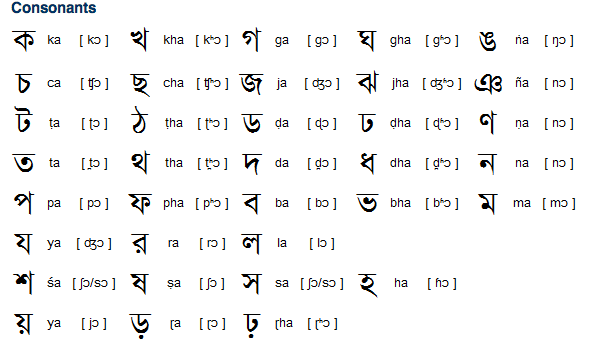
\includegraphics[scale=0.35]{consonants}
  \label{cons}
\end{figure} \\

\section{Past work on Bengali dependency parsing}

Some work has been done in building dependency parsers for Bengali. \citep{ghosh2009dependency} have used a statistical CRF based model followed by a rule based post processing technique. \citep{Nivre_parsingindian}, \citep{ambati_09} used a transition based dependency parsing model based on MaltParser \citep{Nivre05maltparser:a}. \citep{De_Dep_ben} uses a hybrid approach where they simplify the complex and compound sentential structures and then recombine the parses of the simpler structure by satisfying the demands of the verb groups. \citep{bidir_parser} use a bidirectional parser with perceptron learning with rich context as features. \citep{kosaraju_10} used Maltparser and explored the effectiveness of local morphosyntactic features chunk features and automatic semantic information. \citep{attardi_10} used a transition based dependency shift reduce parser which used a Multi layer Perceptron classifier. They were all tested on the same dataset as a part of a shared task held at ICON 2009 and 2010. \citep{husain_09, husain_10}. In the 2009 contest, \citep{ambati_09} system performed the best and in 2010, best score of Unlabeled Attachment Accuracy was achieved by \citep{attardi_10} and the best scores for Label Accuracy and Labeled Attachment was achieved by  \citep{kosaraju_10}.

\section{Existing useful resources for the task}
Microsoft Research India has a POS tagged dataset for several Indian languages including Bengali. The bengali dataset has 899 POS tagged sentences. Also I have been able to gain access to the annotated dataset which was used in the shared task held at ICON 2009 and 2010. Although I am aware that I cannot use the annotated dataset, I am hopeful that it will provide important insights for annotation.

\section{Attested phenomena in the language}
As mentioned earlier Bengali, like many Indian Languages is a free word order language. There has been an annotation effort for dependency parsing in Bengali in the past as a part of the shared task held at ICON 2009 and 2010. The data was annotated using the computational Paninian Grammar \citep{Bharati}. The paninian grammatical model treats a sentence as a series of modifier- modified elements starting from a primary modified (the root of the tree - generally the main verb) \citep{Bharati-2009}. Also in \citep{Bharati-2009} and \citep{Begum-2008}, they have catalogued in detail all the annotation rules. I am planning to follow the same rules just to be consistent, so that my annotations can be reused by researchers. Although the Paninan theory was formulated by Panini (a grammarian from Ancient India) 2500 years ago for the language Sanskrit, it is basically a dependency grammar \citep{Kiparsky, Shastri}. The framework is inspired by a inflectionally rich language such as Sanskrit and gives a strong framework for annotating for other Indian Languages. Also, although \citep{Bharati-2009} has been written as a guideline for annotating Hindi treebank, similar rules should apply to Bengali, because of the similarity in the languages.

\section{Annotations of test corpus}
For the test corpora, I have chosen a dataset of transcribed text of a speech corpus \citep{Shruti}. The text are from news papers and story books. The transcription of the text has been done carefully and is in ITRANS format. I have also found a part of the dataset tagged with the corresponding POS tags. This has really been helpful while annotating for dependencies.

Some of the annotation rule followed:

\begin{enumerate}
\item Multi-word name or proper nouns: In this case, I have made the last word of the name as the root of the chunk and the tree is a linear chain with the first word being the leaf. For example, the proper noun, Mr. Ramesh Singh would become Mr $\leftarrow$ Ramesh $\leftarrow$ Singh.
\item In Bengali, sometimes adverbs are repeated in order to stress something. In this case we again form a linear chain as above. This time the root is the first occurrence of the adverb.
\item Relative clauses - TBD
\item Negative particles: In many cases, negative words normally group with the verb to change the sentence. In Bengali, the negative word usually is after the verb. I have annotated this chunk with the verb as the parent and the negative word as the child.
\item In many cases, Bengali has a lot of multi verb expression (verbs occurring together and expressing the same thing). In such cases I have also annotated the dependency as a linear chain with the head as the first occurring verb.
\item More to be documented.
\end{enumerate}

For the strategy of implementation, I am thinking of doing a  mix of semi-supervised and rule based methods.

\section{First Round of evaluation - System Analysis of corpus A}
I have been able to annotate around \textbf{2500} tokens in total. Separating 2000 tokens for test data, I had around 500 tokens left for training. I used the Turbo Parser \citep{MSXAF10} to train the parser. The features which I used to train the parser are POS tags (coarse and fine). The coarse POS tags are basically the first character of the POS tags. 

 The unlabeled attachment scores after training the basic, standard and full model are listed in table \ref{First}.
\begin{table}
\begin{center}
  \begin{tabular}{ l || c }
  \hline
  Model & Accuracy (\%)\\
  \hline
  Basic Model & \textbf{57.11} \\
  Standard Model & 55.59 \\
  Full Model & 55.27 \\
  \hline
   \end{tabular}
\end{center}
\caption{First round of evaluation on Corpus A. Training size of just 500 tokens}
\label{First}
\end{table}


\section{Lessons learned and Revised Design}
As we can see, the unlabeled accuracies are not that high. This is primarily because of the small size of the training set. Also for the same reason, the basic model is performing better than the standard and the full model. For the next steps, I plan to annotate a lot more data to get meaningful results so that I can think of incorporating other features. Some of the features which I am planning to incorporate are morphological features and also do some unsupervised clustering. But right now, the priority is to annotate more training data.

\subsection{Performance on more training data}
In the few weeks, I have been able to annotate more data for training. Similar features as above were used (coarse and full POS tags). I did annotation in couple of batches. In the first batch, I annotated a total of around \textbf{4000} tokens and at the second round of effort, I was able to annotate around \textbf{5300} tokens. Table \ref{Second} shows the unlabeled attachment scores. \\

The unlabeled accuracy scores are respectable and much better than the initial round of evaluation with just 500 tokens. It is clear that the parser was able to learn better with more training examples. Also the difference in performance of the three models has decreased suggesting that the size of the training set is meaningful to train a standard or full model. Infact for 5300 tokens, the full model performs better than the standard model. Also the difference in accuracies for the two training sets is not much suggesting that we have to use new features to have a better parser. I am planning to add some morphological features to see if there is an increase in the accuracy.\\

As planned earlier, I have incorporated some morphological features of the language. I have used the Bengali morphological analyzer \citep{BMA} made available by the researchers at Indian Institute of Technology Kharagpur. On manual analysis, the performance of the morphological analyzer looked decent. Although there were many morphological features produced as output by the morphological analyzer, I used the root/lemma of a given word as one of the feature. Table \ref{Third} shows the unlabeled accuracy on test corpus A. \\

Morphological features indeed helped!. The accuracy of the parser increased a bit on adding information about the root of each word. This was interesting to observe. Although the performance of the standard model remained the same, the accuracy of both the basic and full model increased. 


\begin{table}
\begin{center}
  \begin{tabular}{ l || c }
  \hline
  Model & Accuracy (\%)\\
  \hline
  Basic Model + 4023 tokens & \textbf{62.32} \\
  Standard Model + 4023 tokens & 60.48 \\
  Full Model + 4023 tokens & 60.91 \\
  Basic Model + 5304 tokens & \textbf{62.98} \\
  Standard Model + 5304 tokens & 61.45 \\
  Full Model + 5304 tokens & 61.89\\
  \hline
   \end{tabular}
\end{center}
\caption{Second round of evaluation on Corpus A.}
\label{Second}
\end{table}



\begin{table}
\begin{center}
  \begin{tabular}{ l || c }
  \hline
  Model & Accuracy (\%)\\
  \hline
  Basic Model + lemma& \textbf{63.74} \\
  Standard Model + lemma& 61.45 \\
  Full Model + lemma& 62.11 \\
  \hline
  Basic Model + l + n + p& 60.59 \\
  Standard Model + l + n + p& 61.89 \\
  Full Model + l + n + p& \textbf{64.17} \\
  \hline
   \end{tabular}
\end{center}
\caption{Unlabeled accuracy on Test Corpus A. Morphological features used for training.}
\label{Third}
\end{table}

\section{System Analysis of Corpus B}

Table \ref{Four} shows the unlabeled accuracy for test corpus B on both the training datasets. On the larger training set, the system performs rather poorly with the highest accuracy of 59.25\% achieved by the full model. As the parser is trained on the larger corpus, the accuracy increased (60.91\% by the full model) though it still performs poorly as compared to test corpus A. 

\begin{table}
\begin{center}
  \begin{tabular}{ l || c }
  \hline
  Model & Accuracy (\%)\\
  \hline
  Basic Model + 4023 tokens & 58.36 \\
  Standard Model + 4023 tokens & 58.14 \\
  Full Model + 4023 tokens & \textbf{59.25} \\
  Basic Model + 5304 tokens & 59.58 \\
  Standard Model + 5304 tokens & \textbf{60.91} \\
  Full Model + 5304 tokens & \textbf{60.91}\\
  \hline
   \end{tabular}
\end{center}
\caption{Unlabeled accuracy on Test Corpus B.}
\label{Four}
\end{table}

\begin{table}
\begin{center}
  \begin{tabular}{ l || c }
  \hline
  Model & Accuracy (\%)\\
  \hline
  Basic Model + lemma & 59.58 \\
  Standard Model + lemma & 61.24 \\
  Full Model + lemma & \textbf{61.90} \\
  \hline
  Basic Model + l + n + p& 59.69 \\
  Standard Model + l + n + p& 60.58 \\
  Full Model + l + n + p& \textbf{61.02} \\
  \hline
   \end{tabular}
\end{center}
\caption{Unlabeled accuracy on Test Corpus B. Morphological features used for training.}
\label{Five}
\end{table}














%Therefore I trained a supervised parser (Turbo Parser) with 1000 training examples. On test dataset A (1000 tokens), it gave an unlabeled attachment score of 41.6$\%$. This is very low and I think because this is primarily because of the very less number of training examples. I plan to annotate a lot more tokens and also try to develop a rule based parser.
 

\newpage


\bibliographystyle{plainnat}
\bibliography{refs}
\label{lastpage}
\end{document}
